\SourcePage{375}{378}
\section{Valence}

The ability of atoms to combine into molecules is described by the concept of \emph{valence}. Each atom is assigned a definite valence, and when atoms combine their valences must saturate one another: every valence bond of one atom must be matched by a valence bond of another. In methane, $\mathrm{CH}_4$, for example, the four valence bonds of the tetravalent carbon atom are saturated by bonds of four monovalent hydrogen atoms. We begin the physical interpretation of valence with the simplest example, the combination of two hydrogen atoms into an $\mathrm H_2$ molecule.

Consider two hydrogen atoms in their ground states (${}^2S$). On approaching, they may form a system in either the ${}^1\Sigma_g^+$ or the ${}^3\Sigma_u^+$ molecular state. The singlet term has an antisymmetric spin wave function, and the triplet term a symmetric one. Conversely, the coordinate wave function is symmetric for the ${}^1\Sigma$ term and antisymmetric for the ${}^3\Sigma$ term. Plainly, only the ${}^1\Sigma$ term can be the ground term of $\mathrm H_2$. Indeed, an antisymmetric wave function $\psi(\mathbf r_1,\mathbf r_2)$, where $\mathbf r_1$ and $\mathbf r_2$ are the radius vectors of the two electrons, necessarily has nodes: it vanishes when $\mathbf r_1=\mathbf r_2$. It therefore cannot describe the lowest state of the system.

Numerical calculation shows that the ${}^1\Sigma$ electronic term does have a deep minimum corresponding to a stable $\mathrm H_2$ molecule. In the ${}^3\Sigma$ state, by contrast, the energy $U(r)$ decreases monotonically as the internuclear distance increases, corresponding to mutual repulsion of the two H atoms\footnote{We disregard here the van der Waals attraction between the atoms (see \S~89). These forces imply that the $U(r)$ curve of the ${}^3\Sigma$ term also has a minimum, located at large distances. This minimum is, however, very shallow compared with that of the ${}^1\Sigma$ curve and would not be visible on the scale of Fig.~29.} (Fig.~29).

\SourcePage{376}{379}
Thus the total spin of the hydrogen molecule in its ground state is zero, $S=0$. The molecules of practically all chemically stable compounds of the main-group elements have this property. Among inorganic molecules, the exceptions are the diatomic molecules $\mathrm O_2$ (ground state ${}^3\Sigma$) and NO (ground state ${}^2\Pi$), and the triatomic molecules $\mathrm{NO}_2$ and $\mathrm{ClO}_2$ (total spin $S=1/2$). The transition-group elements have special properties, to be discussed below after the valence properties of the main-group elements.

\begin{figure}[ht]
\centering
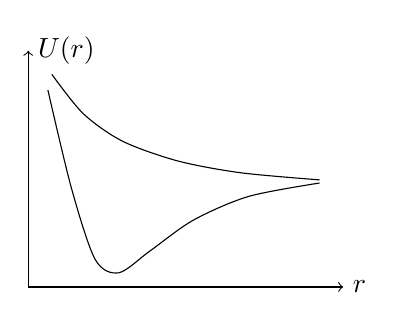
\begin{tikzpicture}[x=1cm,y=1cm]
 \draw[->] (0,0)--(4,0) node[right] {$r$};
 \draw[->] (0,0)--(0,3) node[right] {$U(r)$};
 \draw[smooth] plot coordinates {(.25,2.5)(.55,1.25)(.85,.35)(1.15,.18)(1.55,.46)(2.1,.85)(2.8,1.15)(3.7,1.32)};
 \draw[smooth] plot coordinates {(.3,2.7)(.7,2.2)(1.2,1.85)(1.9,1.6)(2.7,1.45)(3.7,1.36)};
\end{tikzpicture}
\caption*{Fig. 29}
\end{figure}

The ability of atoms to combine is therefore connected with their spin (W.~Heitler, H.~London, 1927). Combination occurs in such a way that the atomic spins compensate one another. A convenient quantitative measure of an atom's ability to combine is the integer equal to twice its spin. This number coincides with the atom's chemical valence. It must be remembered that the same atom may have different valences according to its state.

Consider from this standpoint the main groups of the periodic table. In their normal state the elements of the first group, the first column of Table~3 and the alkali-metal group, have $S=1/2$ and hence valence one. A state of higher spin can be obtained only by exciting an electron from a closed shell. Such states lie so high that the excited atom cannot form a stable molecule\footnote{For Cu, Ag, and Au, see the end of this section.}.

In their normal state, atoms of the second-group elements, the second column of Table~3 and the alkaline-earth group, have $S=0$ and cannot enter chemical compounds in that state. Comparatively close to the ground state, however, there is

\SourcePage{377}{380}
an excited state whose unfilled shell has the configuration $sp$ instead of $s^2$ and whose total spin is $S=1$. The valence in this state is 2, which is the principal valence of the second-group elements.

The normal configuration of the third-group elements is $s^2p$, with $S=1/2$. Excitation of an electron from the filled $s$ shell produces a nearby excited state of configuration $sp^2$ and spin $S=3/2$. These elements accordingly behave as both monovalent and trivalent. The first members of the group, B and Al, are only trivalent. The tendency to show valence 1 grows with atomic number, and Tl is about equally monovalent and trivalent, as in TlCl and $\mathrm{TlCl}_3$. In the first elements of the group, the energetic advantage of the greater binding energy in compounds of the trivalent element, compared with its monovalent compounds, outweighs the excitation energy of the atom.

For the fourth-group elements the ground state has configuration $s^2p^2$ and spin 1, while a nearby excited state has configuration $sp^3$ and spin 2. These states correspond to valences 2 and 4. As in the third group, the first elements C and Si mainly exhibit the higher valence, with CO as an example of an exception, while the tendency toward the lower valence increases with atomic number.

For fifth-group atoms the ground-state configuration is $s^2p^3$, with $S=3/2$, so the corresponding valence is three. A state of higher spin can arise only by transferring an electron to the shell with the next principal quantum number. The nearest such state has configuration $sp^3s'$ and $S=5/2$; here $s'$ denotes an $s$ state whose principal quantum number is one greater than that of $s$. Although its excitation energy is comparatively large, the excited atom can still enter a stable compound. Fifth-group elements are accordingly tri- and pentavalent: nitrogen is trivalent in $\mathrm{NH}_3$ and pentavalent in $\mathrm{HNO}_3$.

For the sixth group, the ground state, of configuration $s^2p^4$, has spin 1 and the atom is divalent. Exciting one $p$ electron gives the state $s^2p^3s'$ with spin 2; exciting one more $s$ electron gives the

\SourcePage{378}{381}
state $sp^3s'p'$ with spin 3. In both excited states the atom can enter stable molecules, exhibiting valences 4 and 6 respectively. The first member, oxygen, shows only valence 2, whereas later members also show the higher valences: sulfur is respectively di-, tetra-, and hexavalent in $\mathrm H_2S$, $\mathrm{SO}_2$, and $\mathrm{SO}_3$.

In the seventh group, the halogens, atoms in the ground state are monovalent, having configuration $s^2p^5$ and spin $S=1/2$. They can also enter stable compounds in excited states with configurations $s^2p^4s'$, $s^2p^3s'p'$, and $sp^3s'p'^2$, whose spins are $3/2$, $5/2$, and $7/2$ and whose valences are 3, 5, and 7. The first element F is always monovalent; later elements also exhibit higher valences. Thus chlorine is respectively mono-, tri-, penta-, and heptavalent in HCl, $\mathrm{HClO}_2$, $\mathrm{HClO}_3$, and $\mathrm{HClO}_4$.

Finally, in their ground states the noble-gas atoms have completely filled shells and $S=0$, while their excitation energies are large. Their valence is accordingly zero and they are chemically inert\footnote{Some nevertheless form stable compounds with fluorine or oxygen. These valences may be connected with transitions of electrons from the outer filled shell to energetically nearby unfilled $f$ or $d$ states.

We also mention a distinctive attraction that arises between a noble-gas atom and an excited atom of the same element. It is connected with the doubling of the number of possible states when two identical atoms in different states are brought together (see \S~80). Transfer of the excitation between the atoms here replaces the exchange interaction that produces ordinary valence. The $\mathrm{He}_2$ molecule is an example. The same type of bond occurs in molecular ions made of two identical atoms, such as $\mathrm H_2^+$.}.

One general qualification applies to all these arguments. To say that an atom enters a molecule with the valence belonging to an excited state does not mean that separating the atoms to large distances must produce an excited atom. It means only that the molecular electron-density distribution around that nucleus is close to the distribution in an isolated excited atom. The limiting distribution as the internuclear distance grows may instead correspond to unexcited atoms.

\SourcePage{379}{382}
When atoms form a molecule, their filled electron shells change little, but the electron density in unfilled shells may change substantially. In the most pronounced instances of the so-called \emph{heteropolar bond}, all valence electrons pass from some atoms to others, so the molecule may be said to consist of ions whose charges, in units of $e$, equal their valences. The first-group elements are electropositive: in heteropolar compounds they give up electrons and form positive ions. Through the later groups electropositivity gradually decreases and becomes electronegativity, strongest in the seventh group. The same qualification applies to heteropolarity as to excited atoms in a molecule. A heteropolar molecule need not yield two ions when separated. CsF would indeed give $\mathrm{Cs}^+$ and $\mathrm F^-$, whereas NaF tends to neutral Na and F atoms, because fluorine's electron affinity exceeds the ionization potential of cesium but is smaller than that of sodium.

In the opposite limiting case, the so-called \emph{homopolar bond}, the atoms remain neutral on average. Unlike heteropolar molecules, homopolar molecules have no appreciable dipole moment. The distinction between the two bond types is purely quantitative, and every intermediate case can occur.

We now turn to the transition-group elements. In their valence properties, the palladium and platinum groups differ little from the main groups. Since their $d$ electrons lie comparatively deep in the atom, however, these electrons interact more weakly with other atoms in a molecule. Consequently, ``unsaturated'' compounds whose molecules have nonzero spin, in fact no greater than $1/2$, are relatively common. Each element may display several valences, differing here by one as well as by two. In the main groups, by contrast, a change of valence results from exciting an electron whose spin was compensated, thereby releasing the spins of a pair of electrons at once.

The rare-earth group is characterized by an unfilled $f$ shell. The $f$ electrons lie much

\SourcePage{380}{383}
deeper than the $d$ electrons and take no part in valence. The valence of a rare-earth element is therefore determined only by the $s$ and $p$ electrons in its unfilled shells\footnote{The $d$ electrons present in unfilled shells of some rare-earth atoms are immaterial, since these atoms in practice always enter compounds in excited states with no $d$ electrons.}. On excitation, however, $f$ electrons may pass into $s$ and $p$ states, increasing the valence by one. Rare-earth elements therefore also show valences differing by one; in practice they are all tri- and tetravalent.

The actinium group occupies a distinctive position. Ac and Th contain no $f$ electrons at all, and their $d$ electrons participate in valence; chemically they therefore resemble the palladium and platinum groups rather than the rare earths. Although a normal U atom contains $f$ electrons, uranium compounds likewise have none. The atoms Np, Pu, Am, and Cm retain $f$ electrons in compounds, but their valence electrons are still $s$ and $d$ electrons; in this sense they are homologous to uranium. The largest possible numbers of unpaired $s$ and $d$ electrons are 1 and 5, respectively, so the maximum valence of the actinium group is six. The corresponding maximum for rare-earth elements, whose $s$ and $p$ electrons participate, is $1+3=4$.

In valence properties the iron group lies between the rare earths and the palladium and platinum groups. Its $d$ electrons are comparatively deep and do not participate in valence bonds in many compounds. In these compounds the iron-group elements behave like rare-earth elements. This includes ionic compounds such as $\mathrm{FeCl}_2$ and $\mathrm{FeCl}_3$, in which the metal atom occurs as a simple cation. Like the rare earths, iron-group elements may exhibit a wide range of valences in such compounds.

Another class is formed by the so-called complex compounds. The transition-element atom then enters the molecule not as a simple ion but as part of a compound, complex ion, for example $\mathrm{MnO}_4^-$ in $\mathrm{KMnO}_4$ or $\mathrm{Fe(CN)}_6^{4-}$ in $\mathrm K_4Fe(CN)_6$. In these complex ions the atoms

\SourcePage{381}{384}
are closer together than in simple ionic compounds, and $d$ electrons participate in the valence bond. The iron-group elements accordingly behave in complex compounds like the palladium and platinum groups.

Finally, Cu, Ag, and Au, assigned to the main groups in \S~73, behave as transition elements in a number of compounds. Their valence can exceed one through promotion of electrons from the $d$ shell into the nearby $p$ shell, for example from $3d$ to $4p$ in Cu. In such compounds the atoms have an unfilled $d$ shell and behave as transition elements: Cu like the iron group, and Ag and Au like the palladium and platinum groups.

\ProblemHeading Determine the electronic terms of the molecular ion $\mathrm H_2^+$ formed by combining a ground-state hydrogen atom with an $\mathrm H^+$ ion, for internuclear distances $R$ large compared with the Bohr radius (L.~D.~Landau, 1961; C.~Herring, 1961)\footnote{For the solution of the analogous problem for $\mathrm H_2$, see L.~P.~Gor'kov, L.~P.~Pitaevskii~// Dokl. Akad. Nauk SSSR. 1963. V.~151. P.~822; C.~Herring, M.~Flicker~// Phys. Rev. 1964. V.~134A. P.~362. The second paper corrects a computational error in the first.}.

\SolutionHeading This problem is analogous in formulation to problem 3 of \S~50: instead of two one-dimensional potential wells, there are two three-dimensional wells around the nuclei, with a common axial symmetry about the line joining them. The level $E_0=-1/2$, the ground level of hydrogen\footnote{Atomic units are used in this problem.}, splits into two levels $U_g(R)$ and $U_u(R)$, the ${}^2\Sigma_g^+$ and ${}^2\Sigma_u^+$ terms, with electronic wave functions
\[
\psi_{g,u}(x,y,z)=\frac1{\sqrt2}[\psi_0(x,y,z)\pm\psi_0(-x,y,z)],
\]
symmetric and antisymmetric with respect to the plane $x=0$ midway between the nuclei, which lie at $x=\pm R/2$ on the $x$ axis. Here $\psi_0(x,y,z)$ is the electron wave function in one of the wells. Exactly as in problem 3 of \S~50,
\begin{equation}U_{g,u}(R)-E_0=\mp\int\psi_0\frac{\partial\psi_0}{\partial x}\,dy\,dz,\tag{1}\end{equation}
where the integration is over the plane $x=0$\footnote{Thus the effect sought is determined by the region of distances where the electron interacts equally with both nuclei.}.

\SourcePage{382}{385}
Seek the function $\psi_0$ corresponding, say, to motion about nucleus 1 at $x=R/2$ in the form
\begin{equation}\psi_0=\frac1{\sqrt\pi}e^{-r_1}a,\tag{2}\end{equation}
where $a$ varies slowly; for an isolated hydrogen atom $a=1$. The function $\psi_0$ obeys
\begin{equation}\frac12\Delta\psi_0+\left(-\frac12-\frac1R+\frac1{r_1}+\frac1{r_2}\right)\psi_0=0,\tag{3}\end{equation}
where $r_1,r_2$ are the distances from the electron to nuclei 1 and 2. The total electronic energy in this equation is $E_0-1/R$, since $E_0$ itself also includes the nuclear Coulomb-repulsion energy $1/R$.

Because $\psi_0$ decreases rapidly away from the $x$ axis, only $y,z\ll R$ matter in (1). For these values, substitution of (2) in (3) gives
\[
\frac{\partial a}{\partial x}+\frac{R/2+x}{R}a=0,
\]
where second derivatives of the slowly varying $a$ have been neglected and $r_2=R/2+x$ has been used. The solution tending to one as $x\to R/2$, near nucleus 1, is
\[
a=\frac{2R}{R+2x}\exp\left(\frac{x}{R}-\frac12\right).
\]
Formula (1) now gives
\[
U_{g,u}-E_0=\mp\frac4e\int_{R/2}^{\infty}e^{-2r_1}2\pi r_1\,dr_1=\mp2Re^{-R-1}.
\]
The splitting is\footnote{The analogous result for $\mathrm H_2$ (see the papers cited above) is $U_g-U_u=-1{,}64R^{5/2}e^{-2R}$.}
\begin{equation}U_g-U_u=-4Re^{-R-1}.\tag{4}\end{equation}

At sufficiently large distances this exponentially decreasing expression becomes smaller than the second-order dipole interaction between H and $\mathrm H^+$. The polarizability of ground-state hydrogen is $9/2$ (see (77.9)), while the field of $\mathrm H^+$ is $\mathcal E=1/R^2$; the corresponding interaction energy is $-9/(4R^4)$. Including it gives
\begin{equation}U_{g,u}(R)-E_0=\mp2Re^{-R-1}-\frac9{4R^4}.\tag{5}\end{equation}
The second term becomes comparable with the first only at $R=10{,}8$. The term $U_u(R)$ also has a minimum at $R=12{,}6$, of depth $-5{,}8\cdot10^{-5}$ atomic units ($-1{,}6\cdot10^{-3}$ eV)\footnote{This van der Waals minimum is very shallow compared with the minimum of $U_g(R)$ corresponding to the normal state of stable $\mathrm H_2^+$. The main minimum occurs at $R=2{,}0$ and has depth $-0{,}60$ atomic units ($-16{,}3$ eV).}.
